% Template latex non officiel pour rapport de TP EEA.
% C'est un template pour thèse que j'ai adapté et 
% auquel j'ai ajouté des éléments au fil du temps pour mes rapports de TP.
% En cas de problèmes n'hésites pas a me contacter.
% David Tocaven
% david.tocaven@gmail.com


%%% /!\ /!\ /!\ /!\ /!\ /!\
% Se compile avec PDFLatex
%%% /!\ /!\ /!\ /!\ /!\ /!\
%%=================================================%%
%%						MAIN
%%=================================================%%


\documentclass[a4paper]{report}

%====================== PACKAGES ======================
\usepackage{bbold}
\usepackage{soul}				% souligner
\usepackage{dsfont}
\usepackage[french]{babel}		% Pour avoir le document en français
\usepackage[utf8x]{inputenc}	% Encodage du document
\usepackage{float}				% Pour gérer les positionnement d'images
\usepackage{amsmath}
\usepackage{mathrsfs}			% Pour les lettres calligraphiques équation
\usepackage[colorinlistoftodos]{todonotes}
\usepackage{url}				% Pour faire des hyperliens vers le web
\usepackage{color}
% pour les informations sur un document compilé en PDF et les liens externes / internes
\usepackage{hyperref}			% Pour faire des hyperliens
\usepackage{array}				% Pour faire des tableaux
\usepackage{tabularx}
% pour utiliser 		% floatbarrier
%\usepackage{placeins}
%\usepackage{floatrow}
\usepackage{setspace}			% Espacement entre les lignes
\usepackage{abstract}			% Modifier la mise en page de l'abstract
\usepackage[T1]{fontenc}		% Police et mise en page (marges) du document
\usepackage[top=2cm, bottom=2cm, left=2cm, right=2cm]{geometry}
\usepackage{pdfpages}			% pour inclures des pdf comme des images
\usepackage{subfig}				% Pour les galerie d'images
\usepackage{listings}			% pour inclure du code dans le doc
\usepackage{soul}				% Pour surligner
\usepackage{enumitem}

\sethlcolor{grisclair}
\definecolor{darkgreen}{RGB}{0,100,0}
%% Titre import from last TP
\usepackage{titlesec, blindtext, color}	
\definecolor{gray75}{gray}{0.75}
\newcommand{\hsp}{\hspace{20pt}}
\titleformat{\chapter}[hang]{\Huge\bfseries}{\thechapter\hsp\textcolor{gray75}{|}\hsp}{0pt}{\Huge\bfseries}


%====================== INFORMATION ET REGLES ======================

%rajouter les numérotation pour les \paragraphe et \subparagraphe
\setcounter{secnumdepth}{4}
\setcounter{tocdepth}{4}

\hypersetup{							% Information sur le document
pdfauthor = { NOM },				% Auteurs
pdftitle = {Matière - Titre - Sujet },		% Titre du document
pdfsubject = {matière},		% Sujet
pdfkeywords = {},				% Mots-clefs
pdfstartview={FitH}}					% ajuste la page à la largueur de l'écran
%pdfcreator = {MikTeX},% Logiciel qui a crée le document
%pdfproducer = {}} % Société avec produit le logiciel

\newcounter{cpt1}						% Compteur pour les n° de ligne dans les prog de l'annexe1
\newcommand\increm{\arabic{cpt1}\addtocounter{cpt1}{1}}
%initialisation de l'intégrateur de language C



%======================== DEBUT DU DOCUMENT ========================

\begin{document}

%\lstset{
%  language=C,                	  % choose the language of the code
%  numbers=left,                   % where to put the line-numbers
%  stepnumber=1,                   % the step between two line-numbers.
%  numbersep=5pt,                  % how far the line-numbers are from the code
%  backgroundcolor=\color{white},  % choose the background color. You must add \usepackage{color}
%  showspaces=false,               % show spaces adding particular underscores
%  showstringspaces=false,         % underline spaces within strings
%  showtabs=false,                 % show tabs within strings adding particular underscores
%  tabsize=2,                      % sets default tabsize to 2 spaces
%  captionpos=b,                   % sets the caption-position to bottom
%  breaklines=true,                % sets automatic line breaking
%  breakatwhitespace=true,         % sets if automatic breaks should only happen at whitespace
%  title=\lstname,                 % show the filename of files included with \lstinputlisting;
%}
%régler l'espacement entre les lignes
\newcommand{\HRule}{\rule{\linewidth}{0.5mm}}


%page de garde
%%=================================================%%
%%						TITRE DU DOCUMENT (1 PAGE)
%							  Pas totalement fini
%%=================================================%%

\begin{titlepage}
\begin{center}

% Upper part of the page. The '~' is needed because only works if a paragraph has started.


\includegraphics[width=0.60\textwidth]{./page_de_garde/logo_ups.png}~\\[1cm]

\textsc{\LARGE Université Paul Sabatier}\\[1.5cm]

\textsc{\Large \bf MATIÈRE }\\[0.5cm]

% Title
\HRule \\[0.4cm]

{\huge \bfseries  - TITRE : \textsc{Sujet} -}

\HRule \\[1.5cm]

% Author and supervisor
\begin{minipage}{0.4\textwidth}
\begin{flushleft} \large
\emph{Auteurs:}\\
%Prenom \textsc{Nom}\\
Prénom \textsc{NOM}\\
\end{flushleft}
\end{minipage}
\begin{minipage}{0.58\textwidth}
\begin{flushright} \large
\emph{Encadrant:} \\
\textbf{ Prénom \textsc{NOM}}
\end{flushright}
\end{minipage}
\newline
\newline

% une éventuelle image
%\includegraphics[width=.6\textwidth]{./page_de_garde/BACDO_schema.pdf}~\\[1cm]

\vfill
% logo fsi & eea
\begin{tabular}{cc}
   
\includegraphics[height=2cm]{./page_de_garde/logo_fsi.png} \hspace{2cm} &
    \hspace{2cm}
   
\includegraphics[height=2cm]{./page_de_garde/logo_eea.jpg} \\
\end{tabular}

% Bottom of the page
{\large \today}

\end{center}
\end{titlepage}
	

%page blanche
\newpage
~
\tableofcontents
\thispagestyle{empty}
\setcounter{page}{0}
%ne pas numéroter le sommaire


%espacement entre les lignes d'un tableau
\renewcommand{\arraystretch}{1.5}

%====================== INCLUSION DES PARTIES ======================
%
%~
\thispagestyle{empty}
%recommencer la numérotation des pages à "1"
\setcounter{page}{0}

\chapter*{Introduction}
\addcontentsline{toc}{chapter}{Introduction}
\label{chap:Intro}	% Importation de introduction.tex

\chapter{Identification-Modélisation du système}
Dans un premier temps, nous allons déterminer les paramètres du moteur, ensuite, nous déterminerons le modèle fréquentiel ainsi que le modèle espace d'état du système. Puis, nous étudierons les propriétés, les performances et la stabilité du système. 
	\section{Détermination de paramètres et du retard}
	On identifiera les paramètres du moteur grâce à une approche dite \emph{boite noire}, c'est-à-dire que suivant la forme d'une réponse du système à un échelon, nous allons choisir une modélisation par fonction de transfert type (1\ier ordre, 2\ieme ordre, ...). Comme il s'agit d'un moteur à courant continu, nous choisissons un modèle du premier ordre car il permet de former un modèle de précision suffisante au vu de notre application.\\
Un modèle du 1\ier ordre est de la forme suivante :
\begin{equation}
G(p) = \frac{K}{\tau p+1}
\end{equation}
Où : 
\begin{description}
\item[$K$ :] Le gain statique du système.
\item[$\tau$ :] La constante de temps du système (en seconde).
\end{description}

\noindent Nous identifierons $K$ en mesurant le gain statique  de la réponse à un signal échelon (pour $t$ tel que la réponse se soit stabilisée): $ K = V_g(t)/U_m(t)$.\\
\noindent Pour l'estimation de $\tau$, nous utiliserons la relation suivante : $ \tau = t$ lorsque $\frac{V_g(t)}{U_m(t)} = 0,63*K $.\\

Pour identifier le retard, que nous savons être sur la commande du moteur, nous allons étudier de déphasage entre un signal d'entrée de type rectangle à fréquence faible ($1$Hz) et la sortie $V_s(t)$. Nous savons analytiquement qu'un système du premier ordre à un déphasage nul à basse fréquence, donc à partir du déphasage mesuré nous pouvons obtenir le retard.

	\section{Autres méthode}
Une autre façon de modéliser le modèle du moteur est un approche de type \emph{boite blanche}, c'est-à-dire de créer un modèle du moteur à partir d'une étude physique du système. 
	\section{Modèle fréquentiel}
Avec l'estimation des paramètres du moteur, nous avons former deux fonctions de transferts. La première définie le la fonction entre $V_g(t)$ et l'entrée $U_m(t)$ et la seconde entre $V_s(t)$ et $U_m(t)$. 
\begin{equation}
\left\lbrace
\begin{array}{l c l }
\frac{V_g(t)}{U_m(t)} 	&=& 	\frac{k_g \cdot k_m}{\tau_m p + 1	}e^{-hp}\\
&&\\
\frac{V_s(t)}{U_m(t)} 	&=& 	\frac{k_s \cdot k_m \cdot k_r}{ p\left(\tau_m p + 1\right)	}e^{-hp}\\
\end{array}
\right.
\end{equation}
Avec l'estimation des paramètres donnés en cours, figure \ref{fig:repIndiFTsEE} tracé (1) , nous avons tracer la réponse à un échelon unité de ces deux fonctions de transferts.
	\section{Modèle espace d'état}
À l'aide des fonctions de transferts précédentes, nous avons fait un modèle espace d'état en choisissant : \\
\begin{description}
\item[Pour entrée $u(t)$ :] $u(t) = U_m(t) $
\item[Pour sorties $y(t)$ :] $ y(t) = \begin{pmatrix}
V_g(t) \\
V_s(t)
\end{pmatrix}$
\item[Pour état $x(t)$ :] $x(t) = \begin{pmatrix}
\Theta_s(t)\\
\Omega_m(t)
\end{pmatrix}$
\end{description}
Nous avons extrait les équations suivantes du modèle schéma-bloc du moteur :
\begin{equation}
\label{eq:VsVgModel}
\left\lbrace
\begin{array}{lcl}
V_g(t) 	&=&		k_g \Omega_m(t)\\
V_s(t) 	&=&		k_s \Theta_s(t)\\
\end{array}
\right.
\end{equation}

Après manipulation des fonctions de transferts précédentes et des expressions de l'équation \ref{eq:VsVgModel}, nous avons obtenu le modèle espace d'état suivant : 
\begin{equation}
\label{eq:EE}
\begin{array}{lcl}

\left\lbrace
\begin{array}{l c l c lc}
\dot{x}(t) 
&=& 
A&
x(t) +& 
B &u(t-h)\\
&&&&\\

y(t) 
&=& 
C&
x(t) +& 
D &u(t-h)\\
\end{array}
\right. 

& \Rightarrow &

\left\lbrace
\begin{array}{l c l c lc}
\dot{x}(t) 
&=& 
\begin{bmatrix}
0	&	k_r\\
0	&	-\frac{1}{\tau_m}
\end{bmatrix}&
x(t) +& 
\begin{bmatrix}
0 \\
\frac{k_m}{\tau_m}
\end{bmatrix} &u(t-h)\\
&&&&\\

y(t) 
&=& 
\begin{bmatrix}
0	&	k_g\\
k_s	&	0
\end{bmatrix}&
x(t) +& 
\begin{bmatrix}
0 \\
0
\end{bmatrix} &u(t-h)\\
\end{array}

\right.
\end{array}
\end{equation}
À l'aide des paramètres de référence, nous avons tracé la réponse à un échelon unité du modèle espace d'état, figuere \ref{fig:repIndiFTsEE}, tracé (2).
\begin{figure}[!ht]
\centering
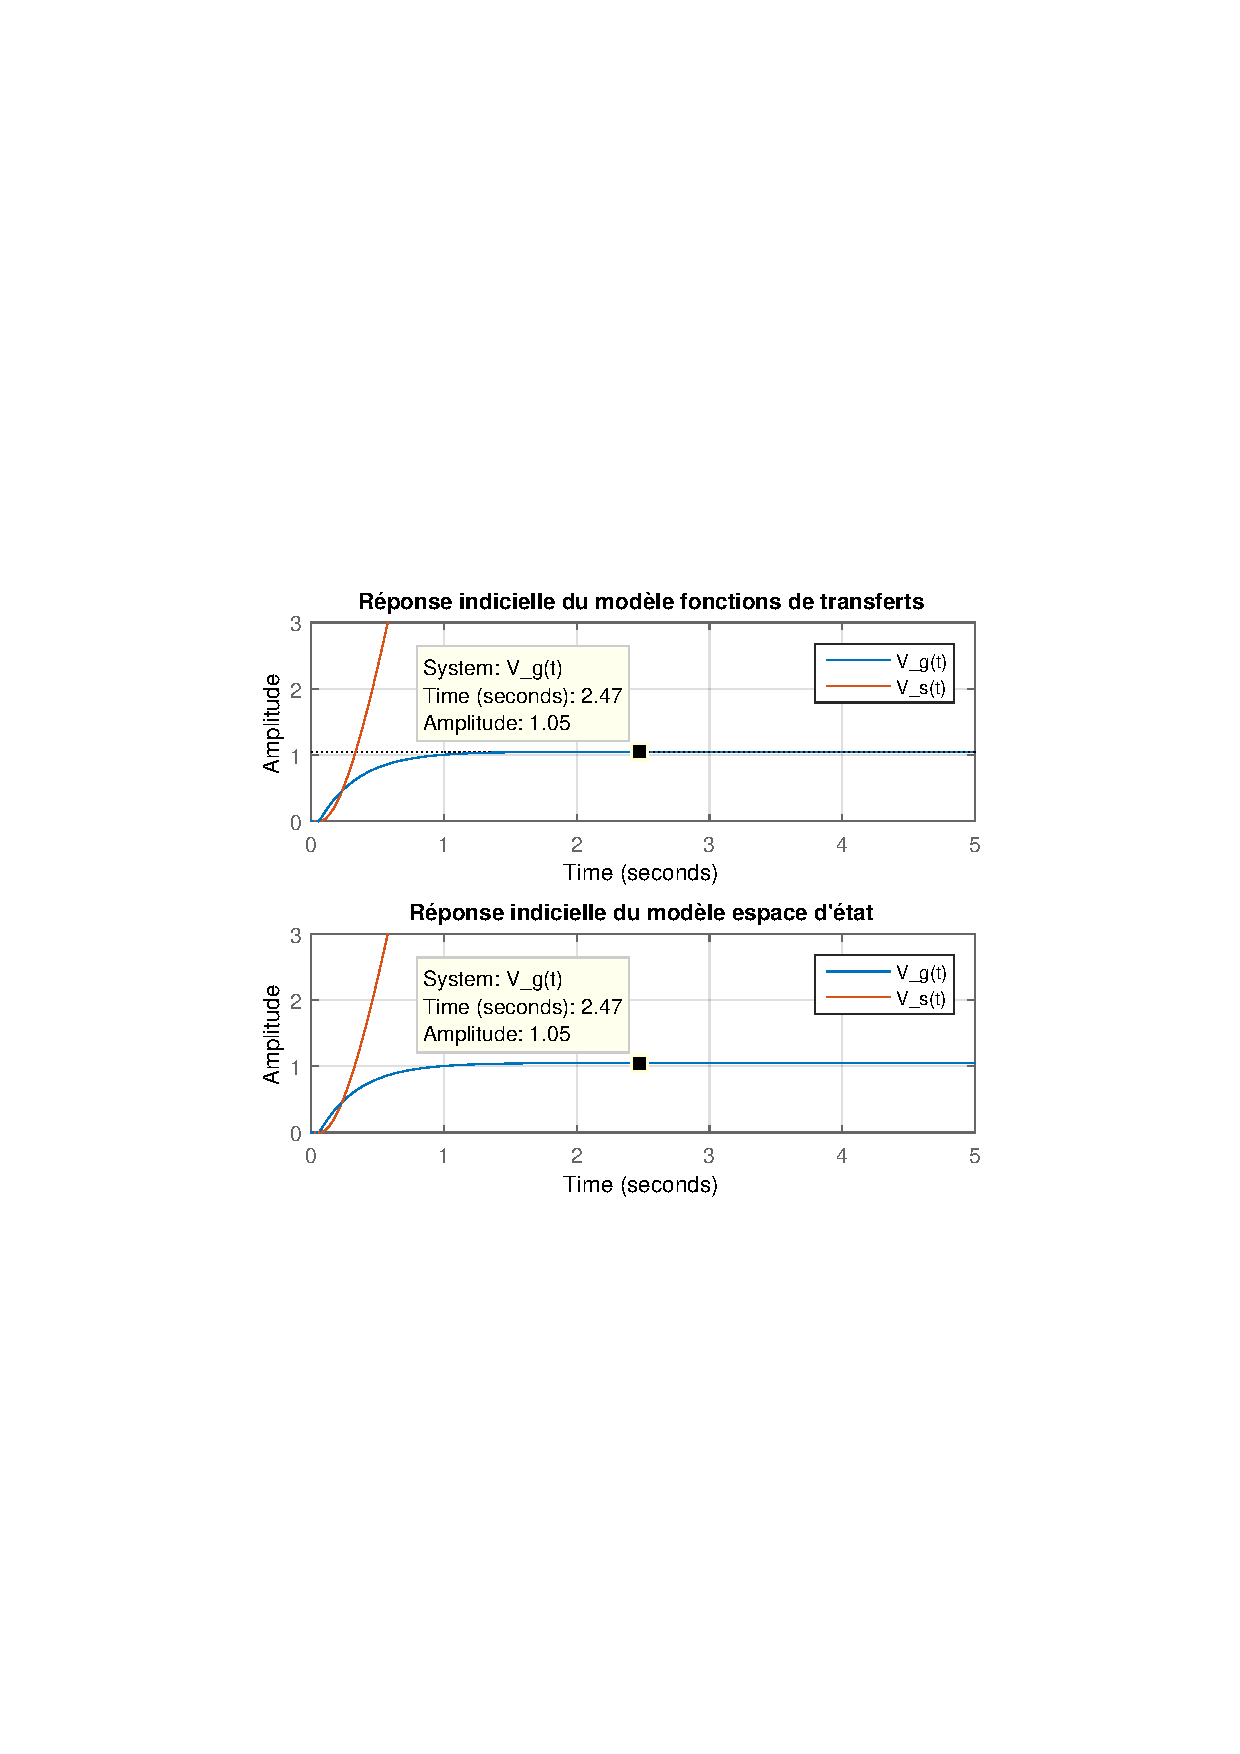
\includegraphics[width=.7\textwidth]{./I/images/modeles_ft-ee.pdf}
\caption{\label{fig:repIndiFTsEE}Réponse à un échelon indiciel des modèles fonctions de transfert (1) et espace d'état (2).}
\end{figure}

Nous avons comparé les réponses entres les deux modélisations afin de vérifier qu'il n'y ai pas d'erreur. Nous avons pour cela tracé la réponse à un échelon unité de la différence des deux modèles, figure \ref{fig:errFT_EE}
\begin{figure}[!ht]
\centering
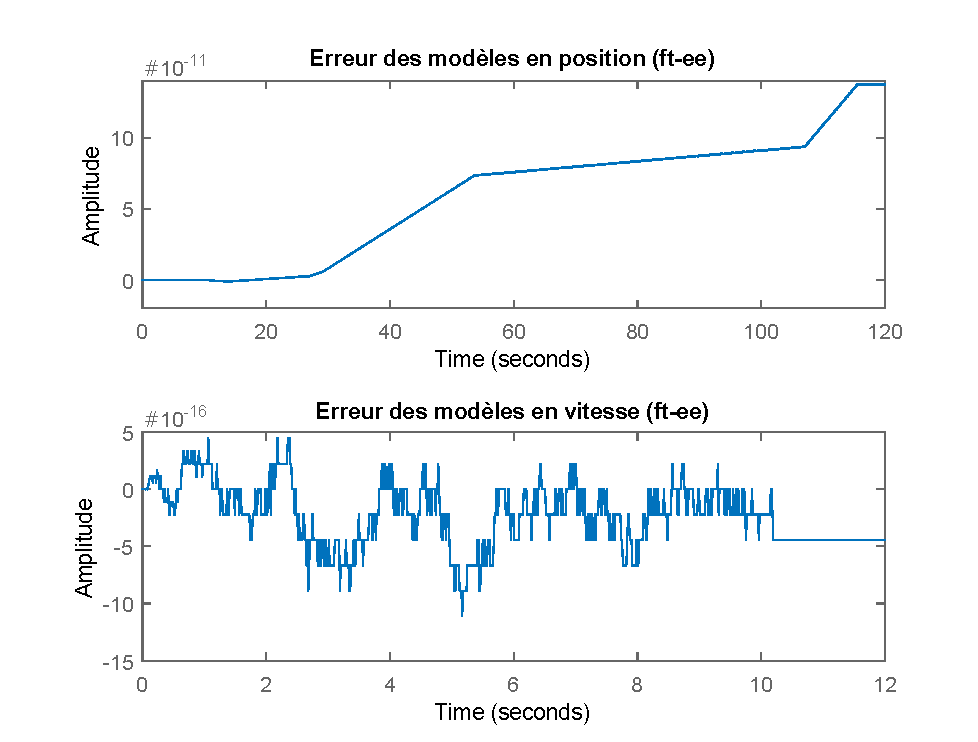
\includegraphics[width=.7\textwidth]{./I/images/erreurs_modeles_ft-ee.pdf}
\caption{\label{fig:errFT_EE} Réponse à un échelon unité de la différence des deux modèles.}
\end{figure}
Nous pouvons constater que l'erreur est négligeable et doit être dût à du bruit numérique et/ou à la méthode de calcul de la réponse. Nos modèles sont donc équivalents par rapport à une réponse à un échelon unité.
	\section{Commandabilité et observabilité}
Nous allons maintenant étudier l'observabilité et la commandabilité de notre modèle. Nous utiliserons, pour cela, le modèle espace d'état et matlab pour résoudre ce point. Nous avons vérifié que le rang de la matrice de commandabilité et de celle d'observabilité sont bien égaux à la dimension de $A$. Ces calculs nous permettent de conclure que le système est observable et commandable.
	\section{Analyse de la boucle ouverte}
Nous allons maintenant étudier les performances de notre système. Nous avons choisi d'étudier les performances sur la sortie $V_g(t)$. 
Toujours à l'aide de matlab, nous avons obtenu les performances suivantes : 
\begin{description}
\item[Temps de monté :] $t_m = 0,659 $ secondes.
\item[Temps de réponse à 5\% :] $t_r = 0,959$ secondes.
\item[Oscillation :] Il n'y a pas d'oscillations.
\item[Gain statique :] $G_{stat}= 1.05$. Il y a donc un dépassement de $0,05$ soit de $5\%$.	
\end{description}	
	\section{Stabilité de la boucle fermée}
	Est-ce bien ces deux méthodes ? (la troisième méthode supposée étant le pseudo-retard non traité en cours)
		\subsection{Delay-Sweeping}
		\subsection{Stabilité 2D}




\chapter{Étude d'une commande Proportionnelle-dérivateur}
\section{Intérêt de ce correcteur}
Pour établir notre asservissement en position, nous devons faire en sorte de commander le transfert entre $u_m$ et $V_s$. Ce transfert dispose d'un intégrateur pur et d'un pôle en $-\frac{1}{\tau _m}$, qui donnent l'instabilité de la position du moteur à une entrée échelon. Un premier correcteur nous est proposé sous la forme :
\begin{equation}\label{eqn:correcteurProportionnel}
C(p) = k_0(1+d_ip)
\end{equation} 
avec $k_0$ le gain proportionnel et $d_i$ le gain dérivateur. Avec une telle correction, nous allons diminué l'ordre du transfert de position/consigne et perdre le pôle en 0 menant à l'instabilité. 

\section{Choix du gain dérivateur du correcteur $C(p)$}
Passons maintenant au choix des valeurs du correcteur. On nous propose un choix particulier pour $d_i$ dans l'énoncé du TP, nous allons voir ensemble en quoi ce choix est judicieux. Nous notons, pour le procédé étudié le transfert $G(p) = \frac{N(p)}{D(p)}=\frac{N(p)}{p(1+\tau_mp)}$, la boucle fermé avec le correcteur en cours d'étude qui intervient de cette manière : 
\begin{align*}
G_{bf}(p) = \frac{Y(p)}{Y_{ref}}	&= \frac{C(p)G(p)}{1+C(p)G(p)} 
										= \frac{k_0(1+d_ip) \frac{N(p)}{D(p)}}{1+k_0(1+d_ip) \frac{N(p)}{D(p)}}	\\
									&= \frac{k_0(1+d_ip) \frac{N(p)}{p(1+\tau_mp)}}{1+ k_0(1+d_ip) \frac{N(p)}{p(1+\tau_mp)}}
\end{align*}
si l'on prend : $d_i = \tau_m$, nous pouvons retomber sur une fonction de transfert plus simple qui est :
\begin{equation}\label{eqn:boucleFermeC_PD}
G_{bf} = \frac{k_0 N(p)}{p+k_0N(p)}
\end{equation}

En sachant que N(p) contient $e^{-hp}$, nous voyons qu'avec ce correcteur, nous allons pouvoir manipuler l'influence du retard dans le système à l'aide $k_0$ et placer le pôle de la boucle fermé corrigé où nous le souhaitons.

\paragraph*{Valeur du gain dérivateur : }\underline{Application numérique} : $d_i = 0.2533$
\section{Choix du gain proportionnel du correcteur $C(p)$}
Maintenant que les calculs théoriques du correcteur ont été effectué, nous allons passer à la recherche du gain proportionnel $k_0$. Pour cela, nous allons à nous référencer aux contraintes du cahier des charges vu en Introduction. Si l'on décompose le résultat établi en \ref{eqn:boucleFermeC_PD}, il vient comme représentation de Laplace du système en boucle fermé :
\begin{equation}\label{eqn:boucleFermeC_PD_detaillé}
G_{bf} = \frac{k_0k_rk_sk_me^{-hp}}{p+k_0k_rk_sk_me^{-hp}}
\end{equation}
Il devient donc évident que l'étude de cette boucle fermé passe par l'étude du quasi-polynôme définit par \begin{equation}\label{eqn:quasipolynome_CPD}
p+k_0k_rk_sk_me^{-hp}=0
\end{equation}

\paragraph*{Valeur du gain proportionnel}
Le cahier des charges nous impose une réponse sans oscillations : cette contrainte est rempli par l'ordre 1 de cette équation caractéristique. Pour remplir les contraintes temporelles et de dépassement, nous allons analyser la boucle fermé obtenu avec un modèle du premier ordre sous la forme : 
\begin{align*}
G(p) = \frac{K}{1+\tau p} &\text{ avec }t_r \text{ le temps de réponse } = 3.3\tau \\& \text{ et } K \text{ le gain en régime établi} 
\end{align*}
en notant tout de même que notre temps de réponse doit être établi à partir du retard du système : $t_r + h \leq 8$. Nous obtenons donc, avec une application numérique : $\tau \leq \frac{8-h}{3.3} \Leftrightarrow \tau \leq 2.42$ et $K=1$. 
Pour une identification de ces paramètres, nous prenons la fonction de transfert en boucle fermé que nous réécrivons pour correspondre avec la forme présentée précédemment : 
\begin{equation}
G_{bf} = \frac{1}{\frac{1}{k_0k_rk_sk_me^{-hp}}p+1}
\end{equation} 
Il vient donc : $\frac{1}{k_0k_rk_sk_me^{-hp}} < 2.42 \Leftrightarrow k_0 > \frac{1}{2.42k_rk_sk_me^{-hp}}$. 

\paragraph*{Valeur gain proportionnel : }\underline{Application numérique} : $k_0 = 0.0354$
\paragraph*{Retard Admissible}
Pour cette étude, nous allons aborder l'étude du quasi-polynôme de la fonction de transfert en boucle fermé établi en `\ref{eqn:quasipolynome_CPD}. 

Nous allons utiliser la méthode du \emph{Delay Sweeping} pour connaitre le retard admissible de notre système en boucle fermé. Pour cela,nous posons :
\begin{equation}\label{eqn:delaySweepingCorPD}
\frac{Q(j\omega)}{P(j\omega)} = \frac{k_0k_sk_mk_r}{j\omega} 
\end{equation}
On obtient alors, pour le calcul du module :
\begin{align}
\norm{\frac{Q(j\omega)}{P(j\omega)}} 	&= \norm{\frac{k_0k_sk_mk_r}{j\omega}} = 1\\
\end{align}
qui donne alors : 
\begin{align*}
\omega= k_0k_sk_mk_r
\end{align*}
Nous appliquons ensuite ce résultat sur le calcul de l'argument suivant pour pouvoir en extraire le retard maximum accessible : 
\begin{align}
&wh^* = -arg\left(-\frac{Q(j\omega)}{P(j\omega)}\right)+2\pi k,\ k \in  \mathbb{Z}
\end{align}
qui nous donne :
\begin{align*}
h^* &= \frac{1}{\omega}arg\left(-\frac{k_0k_sk_rk_m}{j\omega}\right)\\
	&= \frac{1}{\omega}arg(-1)	- arg(j)\ \ \text{     car nous avons noté : } \omega = k_0k_sk_rk_m\\
	&= \frac{\pi}{2 \omega}
\end{align*}

\paragraph*{Valeur retard admissible : }\underline{Application numérique} : $h \in [0; 4.15]$
\section{Calcul de l'erreur de position} 
Avec cette partie, nous pourrons établir l'ajout d'un gain de pré-compensation. Seulement, il vient par construction de l'asservissement la fonction de transfert de la boucle fermé trouvée en \ref{eqn:boucleFermeC_PD_detaillé}. Nous appliquons alors le théorème de la valeur finalesur la sortie du système pour obtenir la valeur du régime permanent. Cette valeur sera ensuite comparé avec la référence (si la référence est égale, tout est bon). Nous avons :
\begin{align*}
\underset{t\rightarrow \infty}{\lim}\ y(t) 	&= \underset{ p\rightarrow 0 }{lim} \ p(Y(p))\\
  											&= \underset{p\rightarrow 0}{lim}\ p(G_{bf}(p)Y_{ref}(p)\\
  											&= \underset{p\rightarrow 0}{lim}\ p \left(\frac{k_0k_rk_sk_me^{-hp}}{p+k_0k_rk_sk_me^{-hp}} \frac{y_{ref}}{p}\right)
\end{align*}
La simplification des variables de Laplace et l'application de leur limite donnent un résultat pour le moins assez trivial qui est :
\begin{align*}
\underset{p\rightarrow 0}{\lim}\ Y(p) = y_{ref}
\end{align*}
donc, nous pouvons conclure sur l'erreur de position en disant : 
\begin{equation}
\underset{t \rightarrow \infty}{lim}\ \epsilon(t) = y(t) - y_{ref}(t) = 0
\end{equation}

\section{Simulation}


\section{Équivalence avec retour d'état instantané}
Pour une loi de commande PD avec comme polynôme $Q(p) = k_1+k_2p+...+k_np^n$ dans la boucle d'asservissement, nous pouvons écrire le développement suivant : 
\begin{align*}
\frac{Y(p)}{E(p)} = \frac{G(p)}{1 + Q(p)G(p)} & \Leftrightarrow \frac{Y(p)}{E(p)} = \frac{Y(p)}{U(p) + Q(p)Y(p)}\\
&\Leftrightarrow \frac{1}{E(p)} = \frac{1}{U(p) + Q(p)Y(p)} \\
& \Leftrightarrow E(p) = U(p) + Q(p)Y(p)\\
& \Leftrightarrow U(p) = E(p) - Q(p)Y(p)
\end{align*} 
Cette dernière ligne est la caractéristique d'un retour d'état, si et seulement si les états sont disponibles sur la sortie du système.

\chapter{Placement du spectre Fini}
Nous allons essayer de développer une loi de commande de dimension infinie permettant d'avoir un système en boucle fermé aillant un spectre fini. Pour cela, nous allons dans un premier temps définir des valeurs de pôles de façon à satisfaire le cahier des charges (voir Introduction). Ensuite, nous allons concevoir la commande de façon à avoir une boucle fermé de spectre fini et remplir le cahier des charges. Dans un troisième temps, nous simulerons le procédé et enfin nous étudierons la robustesse de la commande.

\section{Valeurs des pôles}
Avec le cahier des charges (voir Introduction) nous avons défini que le système en boucle fermé avec le correcteur doit avoir des valeurs propres réelles pour éviter les oscillations. Elles doivent être positives afin que le système soit stable. Avec l'exigence de temps de réponse inférieur ou égale à $8$ secondes, Elles doivent être inférieures ou égalent à $-\frac{1}{8}$. Elles ne doivent être différentes l'une de l'autre afin d'éviter l'instabilité.
Nous avons choisi le valeurs propres suivantes : 
\begin{equation}
vp_{des} = \left\lbrace -\frac{1}{8} -\frac{1}{3} \right\rbrace
\end{equation}
\section{Commande de dimension infinie}
Nous avons ensuite calculer la valeur valeur du correcteur à partir de la forme générale.\\
Nous avons calculer, à partir de l'équation du retour d'état par spectre fini:
\begin{equation}
 u(t) = -K x(t+h)
\end{equation}
Ce retour d'état permet de placer les pôles de notre système en boucle fermé où on le souhaite (ici,celles de la question précédente) et de compenser la partie retardée du modèle du procédé.
À partir du cours, nous avons pris l'équation suivante :
\begin{equation}
x(t+h) = e^{A*h}x(t) + \int_{t}^{t+h} e^{A(t+h-p)}B*u(p-h)dp
\end{equation}
Nous avons effectuer le changement de variable suivant afin d'intégrer de $t-h$ à $t$ : $\phi = p-h$. Cela donne :
\begin{equation}
x(t+h) = e^{Ah} x(t) + \int_{t-h}^{t} e^{A(t-\phi)}Bu(\phi)d\phi
\end{equation}
Nous avons séparer l'exponentielle de la façon à sortir la partie indépendante de $\phi$ de l'intégrale : 
\begin{equation}
x(t+h) = e^{Ah} x(t) + e^{A*t}\int_{t-h}^{t} e^{-A\phi}Bu(\phi)d\phi
\end{equation}
En remplaçant $x(t+h)$ dans l'expression de $u(t)$ précédente : 
\begin{equation}
u(t) = -K \left( e^{Ah} x(t) + e^{A*t}\int_{t-h}^{t} e^{-A\phi}Bu(\phi)d\phi \right)
\end{equation}
Comme il est difficile d'implémenter la fonction de transfert de cette commande sur Simulink, nous laissons cette expression telle qu'elle.
\section{Simulation matlab}
Nous avons simulé le système en boucle fermé ce cette commande sur Simulink et à l'aide de d'un script Matlab. 
Nous avons du décomposer la commande en plusieurs "blocs" que nous avons multiplié et sommé. \\
\begin{description}
\item[$-Ke^{Ah}$ :] Nous avons utilisé un gain dans lequel nous avons utilisé une variable provenant d'un script contenant $e^{Ah}$. Nous avons multiplié l'expression par une matrice $\begin{bmatrix}
0\\
1
\end{bmatrix} $ afin de spécifier qu'il s'agit de la position (car nous asservissons le système en position.
\item[$ e^{At} $ :]  Nous avons utilisé une horloge afin d'avoir $t$, un bloc gain pour A et un bloc \emph{matrix exponential} (\emph{expm})pour avoir l'exponentielle de l'ensemble.
\item[$\int_{t-h}^{t} e^{-A \phi} Bu(\phi)d\phi $ :] Nous avons décomposer cette partie en trois parties : 
\begin{description}
\item[$ e^{-A\phi} $:] La premier partie à intégrer. Nous l'avons fait à partir de $u(t)$ avec un gain contenant $-A$  et un bloc \emph{expm}.
\item[$B*u(\phi)  $ :] La seconde partie à intégrer. Nous l'avons  fait avec un gain contenant $B$ à partir de $u(\phi)$. 
\item[$\int_{t-h}^{t} d\phi $ ] En premier, nous avons multiplié les deux parties précédentes avec un bloc \emph{Matrix Multiply}. Puis, nous avons utilisé un bloc intégrateur pur, à la suite duquel nous avons utiliser un bloc retard paramétré de façon à avoir un retard de $h$ et avons soustrait le signal sortant de l'intégrateur à celui sortant du retard de façon à avoir le signal intégré en $t$ moins le signal en $t-h$.
\end{description}
\item[] Nous avons ensuite multiplié $ e^{At}$ et $\int_{t-h}^{t} e^{-A \phi} Bu(\phi)d\phi $ puis avons multiplié le tout par un gain $-K$. De cette façon, nous réalisons le retour d'état par spectre fini.
\end{description}

Voici le schéma simulink en deux parties, figures \ref{fig:sp1} et \ref{fig:sp2}.

\begin{figure}[!ht]
	\begin{minipage}{.48\textwidth}
		\centering
		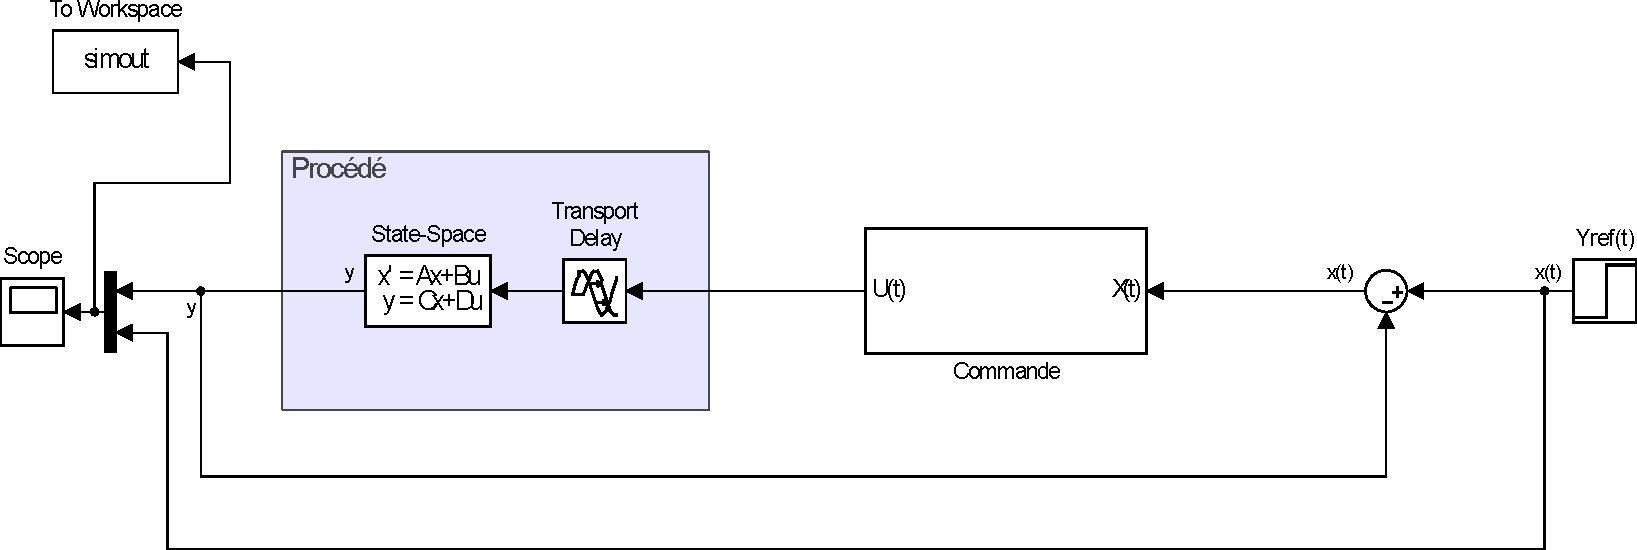
\includegraphics[width=\textwidth]{./III/images/sp1.pdf}
		\caption{\label{fig:sp1}Modèle SIMULINK du système en boucle fermé avec correcteur par retour d'état spectre fini (schéma général).}
	\end{minipage}\hfill
	\begin{minipage}{.48\textwidth}
		\centering
		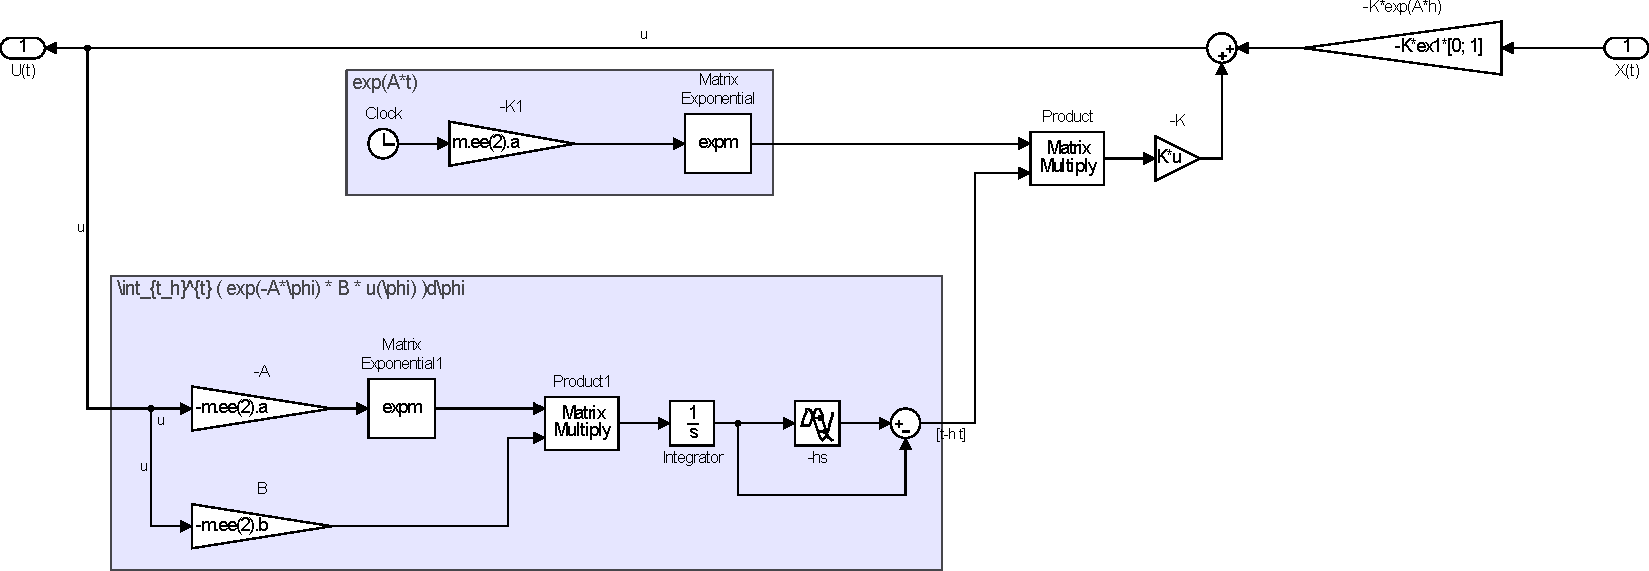
\includegraphics[width=\textwidth]{./III/images/sp2.pdf}
		\caption{\label{fig:sp2}Modèle SIMULINK du système en boucle fermé avec correcteur par retour d'état spectre fini (schéma bloc commande)}
	\end{minipage}
\end{figure}



\section{Robustesse de la commande}
Nous avons testé la commande sur une simulation de très longue durée (400s) et avec un solveur basé sur Euler, on s'aperçoit que le système diverge au bout d'un temps important de simulation ($\approx 300 s$). Cela est dû à l'intégration numérique qui transforme le système, sur un temps long, en un système neutre (voir figure \ref{fig:Vs400}.
\begin{figure}[!ht]
\centering
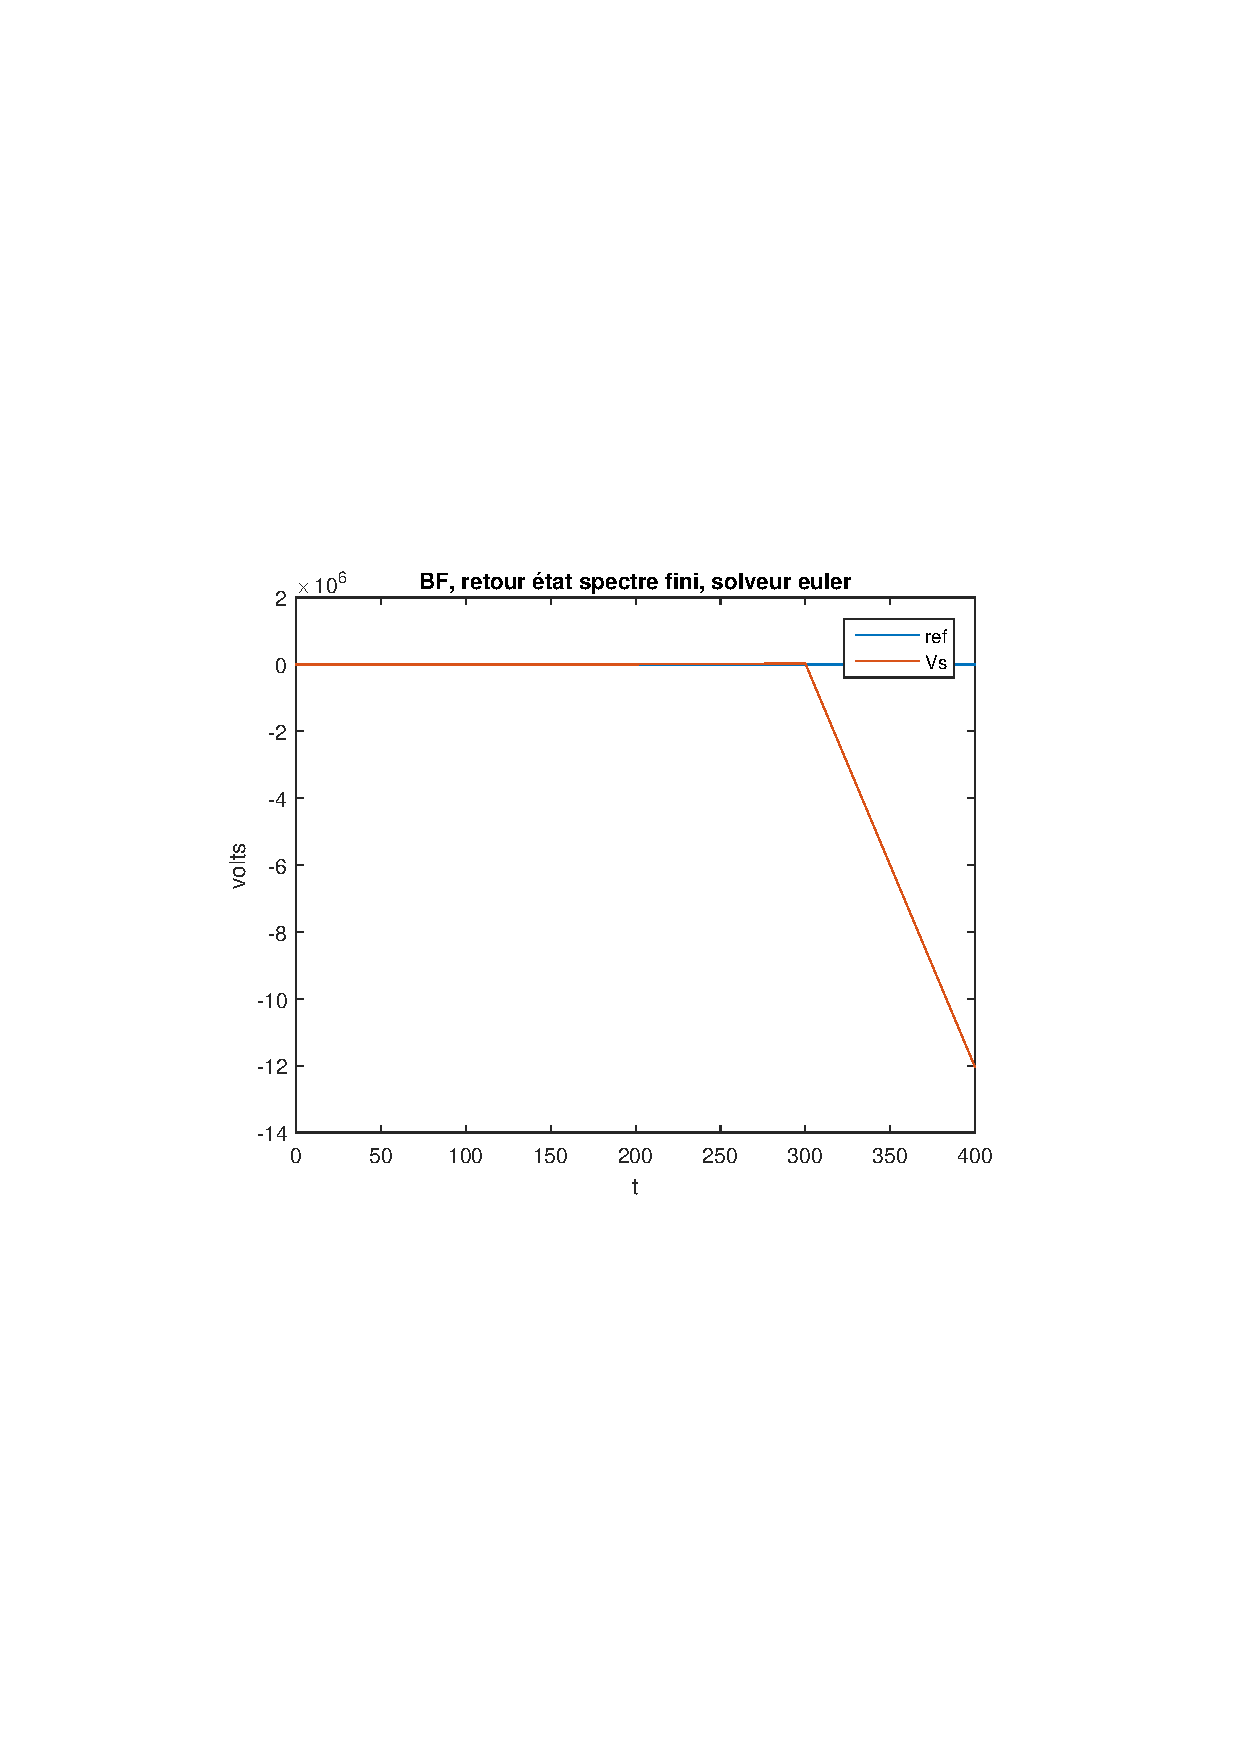
\includegraphics[width=.7\textwidth]{./III/images/Vg_RESpecFini_400.pdf}
\caption{\label{fig:Vs400} Réponse à un échelon unité de la différence des deux modèles.}
\end{figure}


\chapter{Étude d'un prédicteur de Smith}
Nous allons maintenant passer à l'analyse d'un autre type de correction de systèmes à retard : le prédicteur de Smith. Ce type de correcteur permet d'établir une commande de système retardé en utilisant une estimation du procédé qui sera utilisé en temps $t$ et $t+h$.

\section{Schéma de principe du prédicteur de Smith}
Nous avons dessiné avec \emph{Simulink} le schéma bloc en figure \ref{fig:sch_predicteurSmith}, dans lequel nous avons séparé $\tilde{C}(p)$ (C\_Smith sur le schéma) et  $ G(p) e ^{-hp}$(Procédé dans le schéma).
\begin{figure}[!ht]
\centering
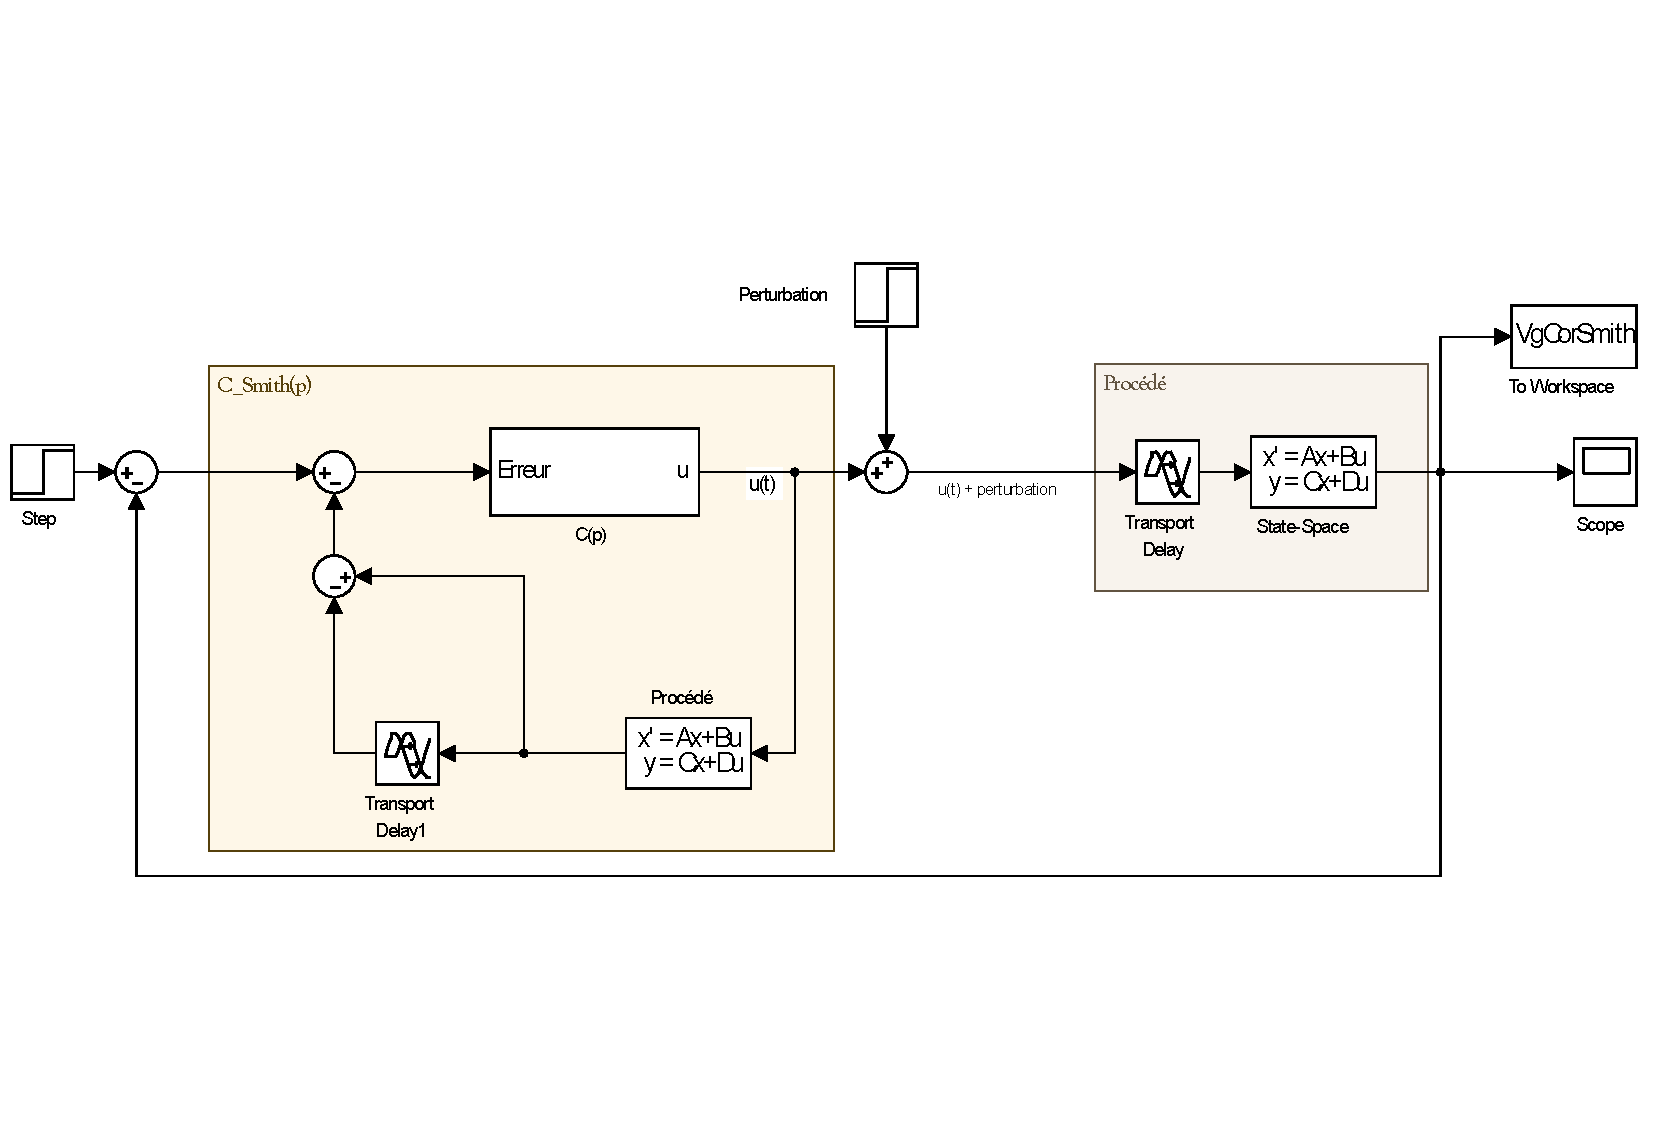
\includegraphics[width=\textwidth]{./IV/images/schema_Predicteur.pdf}
\caption{Schéma de principe du prédicteur de Smith}\label{fig:sch_predicteurSmith}
\end{figure}
Le bloc $C(p)$ devra contenir le bloc de commande que nous souhaitons utiliser. Il pourra être complexe ou bien plus simple.

\section{Fonction de transfert du système en boucle fermé}
Pour obtenir le transfert en boucle fermé de ce schéma, nous allons nous référencer à des résultats de cours et TD, qui sont : 
\begin{equation}
\tilde{C}(p) = \frac{C(p)}{1+G(p)\left(1-e^{-hp}\right)}C(p)	
\end{equation}
ainsi que le transfert de boucle fermé qui s'écrit :
\begin{align}
G_{bf} &= \frac{\tilde{C}G(p)e^{-hp}}{1+\tilde{C}G(p)e^{-hp}}\\
	   &= \frac{C(p)G(p)e^{-hp}}{1+G(p)C(p)}	
\end{align}

Nous utiliserons cette fonction de transfert pour déterminer, à partir du correcteur établi dans les prochaines parties, le polynôme caractéristique du système. 

\section{Correcteur sur le prédicteur de Smith}
On nous propose de mettre un correcteur simple dans la bloc $C(p)$, celui ci sera de a forme : $C(p) = k_0$, soit, un correcteur proportionnel. Nous obtenons avec ce nouvel élément, la fonction de transfert enboucle fermé suivante :
\begin{equation}
G_{bf}(p) = \frac{k_sk_rk_me^{-hp}}{\tau p +p+k_0k_sk_rk_m}
\end{equation}
L'analyse du polynôme caractéristique vient alors dans les équations suivantes :
\begin{align*}
\tau p + p + k_0k_sk_rk_m = 0 \Leftrightarrow p_{1,2} = \frac{-1 \pm \sqrt{1-4\tau k_0k_sk_rk_m}}{2\tau}
\end{align*}
Plusieurs conditions apparaissent alors sur le gain proportionnel pour assurer le cahier des charges : \begin{itemize}
\item [\textbullet]$Re(p_{1,2}) < 0$ pour assurer la stabilité. De cette hypothèse, nous avons alors forcement :\begin{equation}
1-4\tau k_0k_sk_rk_m < 1 \Leftrightarrow k_0 > 0
\end{equation}
Résultat logique, bien qu'il existe des correcteurs avec un gain admis de manière négative, nous sommes ici dans un cas trivial qui n'admet qu'un gain proportionnel positif.
\item [\textbullet] $1-4\tau k_0k_sk_rk_m \geq 0$ pour ne pas avoir des pôles complexes conjugués. Nous avons alors :
\begin{equation}
4\tau k_0k_sk_rk_m \leq 1 \Leftrightarrow k_0 \leq \frac{1}{4\tau k_sk_rk_m}
\end{equation}
\paragraph*{Valeur du Correcteur $C(p)$} \underline{Application numérique} Nous avons alors un correcteur qui est : \begin{equation}\label{eqn:corPredicteurSmith}
C(p) = 0.0925
\end{equation}
\end{itemize}

\chapter{Implantation sur le procédé réel}


%\input{./VI/chap6.tex}

%\input{./conclusions/conclusions.tex}

%\chapter{Conclusion}

%Ne pas numéroter cette partie
\part*{Annexes}
%Rajouter la ligne "Annexes" dans le sommaire
\addcontentsline{toc}{part}{Annexes}

\chapter*{Annexe 1 - TITRE}
\addcontentsline{toc}{chapter}{TITRE}
%\setcounter{section}{0}
% **********************************
\addcontentsline{toc}{section}{TITRE}
\label{Annex:NOM_FICHIER}
\lstset{
  language=Matlab,                	  % choose the language of the code
  basicstyle=\ttfamily,
  numbers=left,                   % where to put the line-numbers
  stepnumber=1,                   % the step between two line-numbers.
  numbersep=5pt,                  % how far the line-numbers are from the code
  backgroundcolor=\color{white},  % choose the background color. You must add \usepackage{color}
  commentstyle = \color{darkgreen},
  showspaces=false,               % show spaces adding particular underscores
  showstringspaces=false,         % underline spaces within strings
  showtabs=false,                 % show tabs within strings adding particular underscores
  tabsize=2,                      % sets default tabsize to 2 spaces
  captionpos=b,                   % sets the caption-position to bottom
  breaklines=true,                % sets automatic line breaking
  breakatwhitespace=true,         % sets if automatic breaks should only happen at whitespace
  %caption=exo1.m,                 % show the filename of files included with \lstinputlisting;
  literate={á}{{\'a}}1 {è}{{\`e}}1 {é}{{\'e}}1,
}
%\lstinputlisting{./annexes/annexe1/NOMFICHIER.m} %{language = MAtlab}
\chapter*{Annexe 2 - TITRE}
\addcontentsline{toc}{chapter}{Annexe 2 - TITRE}
\setcounter{section}{0}
\setcounter{subsection}{0}
% **********************************
	%


\newpage

%récupérer les citation avec "/footnotemark"
\nocite{*}

%%choix du style de la biblio
%\bibliographystyle{unsrt}
%%inclusion de la biblio
%\bibliography{bibliographie}
%%voir wiki pour plus d'information sur la syntaxe des entrées d'une bibliographie

\end{document}

